\chapter{Analyse}
\section{Anforderungsanalyse}

\subsection{Benutzeranforderungen}

Es soll eine Software zur Simulation der zeitlichen Entwicklung einer Temperaturverteilung in Metallplatten entwickelt werden. Diese sollen die Abmessungen 1 Meter x 1 Meter besitzen. Diese können weiterhin inhomogen sein und somit beliebig ortsabhängige Temperaturleitkoeffizienten besitzen. Außerdem ist es dem Benutzer möglich, sowohl die Start- und Randbedingungen des Wärmeleitungsproblems als auch den Endzeitpunkt der Simulation vorzugeben. Des Weiteren ist es dem Benutzer möglich Wärmequellen und deren Intensität ein- sowie weiterhin die Simulationsparameter der Orts- beziehungsweise Zeitdiskretisierung vorzugeben. Jegliche Benutzereingaben erfolgen über eine grafische Oberfläche. Nach Abschluss der Berechnung wird das Ergebnis visualisiert und die zeitliche Entwicklung der Temperaturverteilung kann in Form eines Videos untersucht werden.

%Optional:	Minimierungsproblem „Parameter-Fitting der Wärmeleitkoeffizienten“ im Sinne kleinster Fehlerquadrate lösen, dabei finite Differenzen/automatisches Differenzieren (dco) benutzen.

\subsection{Anwendungsfallanalyse} \label{Kapitel Use Case Analyse}

\subsubsection{Anwendungsfalldiagramm}
Das Anwendungsfalldiagramm zeigt die Abbildung \ref{Use Case Diagramm}.
\begin{figure}[H]
	\centering
	%\hspace{-1.75cm}
	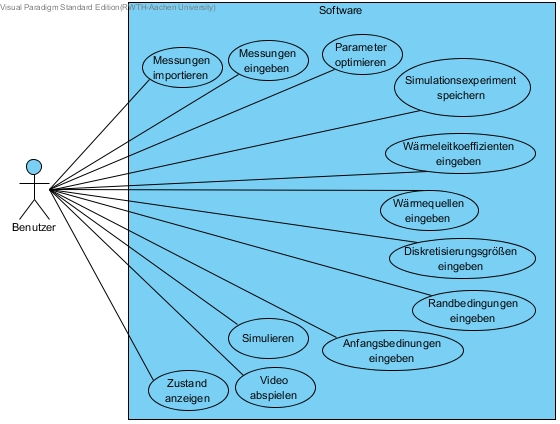
\includegraphics[scale=.6]{Bilder/Use_Case_Diagramm.jpg}\\
	\caption{Anwendungsfalldiagramm}
	\label{Use Case Diagramm}
\end{figure}

\subsubsection{Beschreibungen der Anwendungsfälle}
Die folgenden Tabellen (Tab. \ref{Beschreibung Use Case Anfangsbedingungen eingeben} - \ref{Beschreibung Use Case Zustand anzeigen}) zeigen die Beschreibungen der Anwendungsfälle.

%Anfangsbedingungen_eingeben
\begin{table} [H]
	\centering
	%\hspace{-1cm}
	\begin{tabular}{|l|l|l|}
		\hline
		\textbf{Name} 			& \multicolumn{2}{|l|}{Anfangsbedingungen eingeben}  \\
		\hline
		\textbf{Ziel} 			& \multicolumn{2}{|l|}{Der Benutzer möchte Anfangsbedingungen vorgeben. }\\ 
		\hline
		\textbf{Einordnung}		& \multicolumn{2}{|l|}{Hauptfunktion}\\
		\hline
		\textbf{Vorbedingung}	& \multicolumn{2}{|l|}{Die Software wird korrekt ausgeführt.} \\
		\hline
		\textbf{Nachbedingung}	& \multicolumn{2}{|l|}{Die Anfangsbedingungen wurden vorgegeben und gespeichert.}\\
		\hline
		\textbf{Nachbedingung} 	& \multicolumn{2}{|l|}{Die Anfangsbedingungen wurden nicht geändert und}\\
		\textbf{im Fehlerfall}	& \multicolumn{2}{|l|}{entsprechende Fehlermeldungen wurden ausgegeben.}\\
		\hline
		\textbf{Haupt-} 			& \multicolumn{2}{|l|}{Benutzer}\\
		\textbf{Neben-Akteur}	& \multicolumn{2}{|l|}{	}			\\
		\hline
		\textbf{Auslöser} 		& \multicolumn{2}{|l|}{Der Benutzer möchte Anfangsbedingungen vorgeben.} \\
		\hline 
		\textbf{Standardfluss} & \textbf{Schritt} & \textbf{Aktion} \\
		\hline
		&	1	& Der Benutzer wählt den Menüpunkt \emph{Anfangsbedingungen} aus. \\
		\cline{2-3}
		&	2	& Die Software wechselt zu dem entsprechenden Menü.\\
		\cline{2-3}
		&	3	& Der Benutzer gibt die Anfangsbedingungen vor.\\
		\cline{2-3}
		&	4	& Die Software prüft die eingegebenen Anfangsbedingungen.\\
		\cline{2-3}
		&	5	& Die Software speichert die Anfangsbedingungen.\\
		\hline
		\textbf{Nebenfluss} & \textbf{Schritt} & \textbf{Aktion}\\
		\hline
		Anfangsbedingung-  & 5a.1 & Eine Fehlermeldung wird angezeigt.\\
		\cline{2-3}
		en nicht akzeptiert 	& 5a.2	& Der Benutzer korrigiert seine Eingabe.\\
		\cline{2-3}
					& 5a.3 	& $\rightarrow$ Schritt 4\\
		\hline
	\end{tabular}
	\caption{Beschreibung Use Case Anfangsbedingungen eingeben}
	\label{Beschreibung Use Case Anfangsbedingungen eingeben}
\end{table}

%Diskretisierungsgrößen_eingeben
\begin{table} [H]
	\centering
	%\hspace{-1cm}
	\begin{tabular}{|l|l|l|}
		\hline
		\textbf{Name} 			& \multicolumn{2}{|l|}{Diskretisierungsgrößen eingeben}  \\
		\hline
		\textbf{Ziel} 			& \multicolumn{2}{|l|}{Der Benutzer möchte Diskretisierungsgrößen eingeben. }\\ 
		\hline
		\textbf{Einordnung}		& \multicolumn{2}{|l|}{Hauptfunktion}\\
		\hline
		\textbf{Vorbedingung}	& \multicolumn{2}{|l|}{Die Software wird korrekt ausgeführt.} \\
		\hline
		\textbf{Nachbedingung}	& \multicolumn{2}{|l|}{Die Diskretisierungsgrößen wurden vorgegeben und gespeichert.}\\
		\hline
		\textbf{Nachbedingung} 	& \multicolumn{2}{|l|}{Die Diskretisierungsgrößen wurden nicht geändert und}\\
		\textbf{im Fehlerfall}	& \multicolumn{2}{|l|}{entsprechende Fehlermeldungen wurden ausgegeben.}\\
		\hline
		\textbf{Haupt-} 		& \multicolumn{2}{|l|}{Benutzer}\\
		\textbf{Neben-Akteur}	& \multicolumn{2}{|l|}{	}			\\
		\hline
		\textbf{Auslöser} 		& \multicolumn{2}{|l|}{Der Benutzer möchte Diskretisierungsgrößen eingeben.} \\
		\hline 
		\textbf{Standardfluss} & \textbf{Schritt} & \textbf{Aktion} \\
		\hline
		&	1	& Der Benutzer wählt den Menüpunkt \emph{Diskretisierungsgrößen} aus. \\
		\cline{2-3}
		&	2	& Die Software wechselt zu dem entsprechenden Menü.\\
		\cline{2-3}
		&	3	& Der Benutzer gibt die Stützstellenzahl der Ortsdiskretisierung \emph{n} ein.\\
		\cline{2-3}
		&	4	& Der Benutzer gibt die Stützstellenzahl der Zeitdiskretisierung \emph{m} ein.\\
		\cline{2-3}
		&	5	& Der Benutzer gibt den Endzeitpunkt \emph{T} ein.\\
		\cline{2-3}
		&	6	& Die Software prüft die eingegebenen Größen.\\
		\cline{2-3}
		&	7	& Die Software speichert die eingegebenen Größen.\\
		\hline
		\textbf{Nebenfluss} & \textbf{Schritt} & \textbf{Aktion}\\
		\hline
		Eingegebene Größ-  & 7a.1 & Eine Fehlermeldung wird angezeigt.\\
		\cline{2-3}
		en nicht akzeptiert & 7a.2	& Der Benutzer korrigiert seine Eingabe.\\
		\cline{2-3}
					& 7a.3 	& $\rightarrow$ Schritt 6\\
		\hline
	\end{tabular}
	\caption{Beschreibung Use Case Diskretisierungsgrößen eingeben}
	\label{Beschreibung Use Case Diskretisierungsgrössen eingeben}
\end{table}

%Randbedingungen_eingeben
\begin{table} [H]
	\centering
	%\hspace{-1cm}
	\begin{tabular}{|l|l|l|}
		\hline
		\textbf{Name} 			& \multicolumn{2}{|l|}{Randbedingungen eingeben}  \\
		\hline
		\textbf{Ziel} 			& \multicolumn{2}{|l|}{Der Benutzer möchte Randbedingungen vorgeben. }\\ 
		\hline
		\textbf{Einordnung}		& \multicolumn{2}{|l|}{Hauptfunktion}\\
		\hline
		\textbf{Vorbedingung}	& \multicolumn{2}{|l|}{Die Software wird korrekt ausgeführt.} \\
		\hline
		\textbf{Nachbedingung}	& \multicolumn{2}{|l|}{Die Randbedingungen wurden vorgegeben und gespeichert.}\\
		\hline
		\textbf{Nachbedingung} 	& \multicolumn{2}{|l|}{Die Randbedingungen wurden nicht geändert und}\\
		\textbf{im Fehlerfall}	& \multicolumn{2}{|l|}{entsprechende Fehlermeldungen wurden ausgegeben.}\\
		\hline
		\textbf{Haupt-} 			& \multicolumn{2}{|l|}{Benutzer}\\
		\textbf{Neben-Akteur}	& \multicolumn{2}{|l|}{	}			\\
		\hline
		\textbf{Auslöser} 		& \multicolumn{2}{|l|}{Der Benutzer möchte Randbedingungen vorgeben.} \\
		\hline 
		\textbf{Standardfluss} & \textbf{Schritt} & \textbf{Aktion} \\
		\hline
		&	1	& Der Benutzer wählt den Menüpunkt \emph{Randbedingungen} aus. \\
		\cline{2-3}
		&	2	& Die Software wechselt zu dem entsprechenden Menü.\\
		\cline{2-3}
		&	3	& Der Benutzer gibt die Randbedingungen vor.\\
		\cline{2-3}
		&	4	& Die Software prüft die eingegebenen Randbedingungen.\\
		\cline{2-3}
		&	5	& Die Software speichert die Randbedingungen.\\
		\hline
		\textbf{Nebenfluss} & \textbf{Schritt} & \textbf{Aktion}\\
		\hline
		Randbedingungen  & 5a.1 & Eine Fehlermeldung wird angezeigt.\\
		\cline{2-3}
		nicht akzeptiert 	& 5a.2	& Der Benutzer korrigiert seine Eingabe.\\
		\cline{2-3}
					& 5a.3 	& $\rightarrow$ Schritt 4\\
		\hline
	\end{tabular}
	\caption{Beschreibung Use Case Randbedingungen eingeben}
	\label{Beschreibung Use Case Randbedingungen eingeben}
\end{table}

%Simulieren
\begin{table} [H]
        \centering
        %\hspace{-1cm}
        \begin{tabular}{|l|l|l|}
                \hline
                \textbf{Name}           & \multicolumn{2}{|l|}{Simulieren}  \\
                \hline
                \textbf{Ziel}           & \multicolumn{2}{|l|}{Der Benutzer möchte simulieren. }\\ 
                \hline
                \textbf{Einordnung}     & \multicolumn{2}{|l|}{Hauptfunktion}\\
                \hline
                \textbf{Vorbedingung}   & \multicolumn{2}{|l|}{Die Software wird korrekt ausgeführt.} \\
                \hline
                \textbf{Nachbedingung}  & \multicolumn{2}{|l|}{Die Simulation wurde ausgeführt.}\\
                \hline
                \textbf{Nachbedingung}  & \multicolumn{2}{|l|}{Die Simulation wurden nicht ausgeführt und}\\
                \textbf{im Fehlerfall}  & \multicolumn{2}{|l|}{entsprechende Fehlermeldungen wurden ausgegeben.}\\
                \hline
                \textbf{Haupt-}                         & \multicolumn{2}{|l|}{Benutzer}\\
                \textbf{Neben-Akteur}   & \multicolumn{2}{|l|}{ }                       \\
                \hline
                \textbf{Auslöser}               & \multicolumn{2}{|l|}{Der Benutzer möchte die Simulation starten.} \\
                \hline 
                \textbf{Standardfluss} & \textbf{Schritt} & \textbf{Aktion} \\
                \hline
                &		1		& Der Benutzer wählt den Menüpunkt \emph{Simulieren} aus. \\
				\cline{2-3}
				&		2		& Die Software wechselt zu dem entsprechenden Menü.\\
				\cline{2-3}
                &       3 		& Der Benutzer drückt den Knopf \emph{Simulieren}. \\
                \cline{2-3}
                &       4       & Die Software simuliert.\\
                \cline{2-3}
                &       5       & Die Software wechselt zu dem Menü \emph{Visualisierung}.\\
                \cline{2-3}
                &       6      & Die Software stellt den Endzustand dar.\\
                \hline
        \end{tabular}
        \caption{Beschreibung Use Case Simulieren}
        \label{Beschreibung Use Case Simulieren}
\end{table}

%Video_abspielen
\begin{table} [H]
	\centering
	%\hspace{-1cm}
	\begin{tabular}{|l|l|l|}
		\hline
		\textbf{Name} 			& \multicolumn{2}{|l|}{Video abspielen}  \\
		\hline
		\textbf{Ziel} 			& \multicolumn{2}{|l|}{Der Benutzer möchte die zeitliche Entwicklung der Temperaturverteilung  }\\ 
		& \multicolumn{2}{|l|}{untersuchen.}\\
		\hline
		\textbf{Einordnung}		& \multicolumn{2}{|l|}{Hauptfunktion}\\
		\hline
		\textbf{Vorbedingung}	& \multicolumn{2}{|l|}{Die Software wird korrekt ausgeführt und es wurde eine Simulation} \\
		& \multicolumn{2}{|l|}{ erfolgreich durchgeführt.} \\
		\hline
		\textbf{Nachbedingung}	& \multicolumn{2}{|l|}{Das Video wird abgespielt.}\\
		\hline
		\textbf{Nachbedingung} 	& \multicolumn{2}{|l|}{Das Video wurde nicht abgespielt und}\\
		\textbf{im Fehlerfall}	& \multicolumn{2}{|l|}{entsprechende Fehlermeldungen wurden ausgegeben.}\\
		\hline
		\textbf{Haupt-} 		& \multicolumn{2}{|l|}{Benutzer}\\
		\textbf{Neben-Akteur}	& \multicolumn{2}{|l|}{	}			\\
		\hline
		\textbf{Auslöser} 		& \multicolumn{2}{|l|}{Der Benutzer möchte die zeitliche Entwicklung der Temperaturverteilung} \\
		& \multicolumn{2}{|l|}{untersuchen.}\\
		\hline 
		\textbf{Standardfluss} & \textbf{Schritt} & \textbf{Aktion} \\
		\hline
		&	1	& Der Benutzer wählt den Menüpunkt \emph{Visualisierung} aus. \\
		\cline{2-3}
		&	2	& Die Software wechselt zu dem entsprechenden Menü.\\
		\cline{2-3}
		&	3	& Der Benutzer startet das Video.\\
		\cline{2-3}
		&	4	& Die Software spielt das Video ab.\\
		\hline
	\end{tabular}
	\caption{Beschreibung Use Case Video abspielen}
	\label{Beschreibung Use Case Video abspielen}
\end{table}

%Wärmeleitkoeffizienten_eingeben
\begin{table} [H]
	\centering
	%\hspace{-1cm}
	\begin{tabular}{|l|l|l|}
		\hline
		\textbf{Name} 			& \multicolumn{2}{|l|}{Wärmeleitkoeffizienten eingeben}  \\
		\hline
		\textbf{Ziel} 			& \multicolumn{2}{|l|}{Der Benutzer möchte Wärmeleitkoeffizienten eingeben. }\\ 
		\hline
		\textbf{Einordnung}		& \multicolumn{2}{|l|}{Hauptfunktion}\\
		\hline
		\textbf{Vorbedingung}	& \multicolumn{2}{|l|}{Die Software wird korrekt ausgeführt.} \\
		\hline
		\textbf{Nachbedingung}	& \multicolumn{2}{|l|}{Die Wärmeleitkoeffizienten wurden eingegeben und gespeichert.}\\
		\hline
		\textbf{Nachbedingung} 	& \multicolumn{2}{|l|}{Die Wärmeleitkoeffizienten wurden nicht geändert und}\\
		\textbf{im Fehlerfall}	& \multicolumn{2}{|l|}{entsprechende Fehlermeldungen wurden ausgegeben.}\\
		\hline
		\textbf{Haupt-} 			& \multicolumn{2}{|l|}{Benutzer}\\
		\textbf{Neben-Akteur}	& \multicolumn{2}{|l|}{	}			\\
		\hline
		\textbf{Auslöser} 		& \multicolumn{2}{|l|}{Der Benutzer möchte Wärmeleitkoeffizienten eingeben.} \\
		\hline 
		\textbf{Standardfluss} & \textbf{Schritt} & \textbf{Aktion} \\
		\hline
		&	1	& Der Benutzer wählt den Menüpunkt \emph{Wärmeleitkoeffizienten} aus. \\
		\cline{2-3}
		&	2	& Die Software wechselt zu dem entsprechenden Menü.\\
		\cline{2-3}
		&	3	& Der Benutzer wählt auf der Darstellung der Platte die \\
		&       & gewünschten Gebiete.\\
		\cline{2-3}
		&	4	& Die Software prüft die eingegebenen Gebiete.\\
		\cline{2-3}
		&	5	& Der Benutzer wählt die Werte für die einzelnen Gebiete.\\
		\cline{2-3}
		&	6	& Die Software prüft die eingegebenen Werte.\\
		\cline{2-3}
		&	7	& Die Software speichert die Gebiete und die Werte.\\
		\hline
		\textbf{Nebenfluss} & \textbf{Schritt} & \textbf{Aktion}\\
		\hline
		Gebiet nicht & 5a.1 & Eine Fehlermeldung wird angezeigt.\\
		\cline{2-3}
		akzeptiert 	& 5a.2	& Der Benutzer korrigiert seine Eingabe.\\
		\cline{2-3}
					& 5a.3 	& $\rightarrow$ Schritt 4\\
		\hline
		Werte nicht & 7a.1 	& Eine Fehlermeldung wird angezeigt.\\
		\cline{2-3}
		akzeptiert 	& 7a.2	& Der Benutzer korrigiert seine Eingabe.\\
		\cline{2-3}
					& 7a.3 	& $\rightarrow$ Schritt 6\\
		\hline
	\end{tabular}
	\caption{Beschreibung Use Case Wärmeleitkoeffizienten eingeben}
	\label{Beschreibung Use Case Wärmeleitkoeffizienten eingeben}
\end{table}

%Wärmequellen_eingeben
\begin{table} [H]
	\centering
	%\hspace{-1cm}
	\begin{tabular}{|l|l|l|}
		\hline
		\textbf{Name} 			& \multicolumn{2}{|l|}{Wärmequellen eingeben}  \\
		\hline
		\textbf{Ziel} 			& \multicolumn{2}{|l|}{Der Benutzer möchte Wärmequellen eingeben. }\\ 
		\hline
		\textbf{Einordnung}		& \multicolumn{2}{|l|}{Hauptfunktion}\\
		\hline
		\textbf{Vorbedingung}	& \multicolumn{2}{|l|}{Die Software wird korrekt ausgeführt.} \\
		\hline
		\textbf{Nachbedingung}	& \multicolumn{2}{|l|}{Die Wärmequellen wurden eingegeben und gespeichert.}\\
		\hline
		\textbf{Nachbedingung} 	& \multicolumn{2}{|l|}{Die Wärmequellen wurden nicht geändert und}\\
		\textbf{im Fehlerfall}	& \multicolumn{2}{|l|}{entsprechende Fehlermeldungen wurden ausgegeben.}\\
		\hline
		\textbf{Haupt-} 			& \multicolumn{2}{|l|}{Benutzer}\\
		\textbf{Neben-Akteur}	& \multicolumn{2}{|l|}{	}			\\
		\hline
		\textbf{Auslöser} 		& \multicolumn{2}{|l|}{Der Benutzer möchte Wärmequellen eingeben.} \\
		\hline 
		\textbf{Standardfluss} & \textbf{Schritt} & \textbf{Aktion} \\
		\hline
		&	1	& Der Benutzer wählt den Menüpunkt \emph{Wärmequellen} aus. \\
		\cline{2-3}
		&	2	& Die Software wechselt zu dem entsprechenden Menü.\\
		\cline{2-3}
		&	3	& Der Benutzer wählt auf der Darstellung der Platte die \\
		&       & gewünschten Gebiete.\\
		\cline{2-3}
		&	4	& Die Software prüft die eingegebenen Gebiete.\\
		\cline{2-3}
		&	5	& Der Benutzer wählt die Werte für die einzelnen Gebiete.\\
		\cline{2-3}
		&	6	& Die Software prüft die eingegebenen Werte.\\
		\cline{2-3}
		&	7	& Die Software speichert die Gebiete sowie die Werte.\\
		\hline
		\textbf{Nebenfluss} & \textbf{Schritt} & \textbf{Aktion}\\
		\hline
		Gebiet nicht & 5a.1 & Eine Fehlermeldung wird angezeigt.\\
		\cline{2-3}
		akzeptiert 	& 5a.2	& Der Benutzer korrigiert seine Eingabe.\\
		\cline{2-3}
					& 5a.3 	& $\rightarrow$ Schritt 4\\
		\hline
		Werte nicht & 7a.1 	& Eine Fehlermeldung wird angezeigt.\\
		\cline{2-3}
		akzeptiert 	& 7a.2	& Der Benutzer korrigiert seine Eingabe.\\
		\cline{2-3}
					& 7a.3 	& $\rightarrow$ Schritt 6\\
		\hline
	\end{tabular}
	\caption{Beschreibung Use Case Wärmequellen eingeben}
	\label{Beschreibung Use Case Wärmequellen eingeben}
\end{table}

%Zustand_anzeigen
\begin{table} [H]
	\centering
	%\hspace{-1cm}
	\begin{tabular}{|l|l|l|}
		\hline
		\textbf{Name} 			& \multicolumn{2}{|l|}{Zustand anzeigen}  \\
		\hline
		\textbf{Ziel} 			& \multicolumn{2}{|l|}{Der Benutzer möchte ein Zustand anzeigen lassen. }\\ 
		\hline
		\textbf{Einordnung}		& \multicolumn{2}{|l|}{Hauptfunktion}\\
		\hline
		\textbf{Vorbedingung}	& \multicolumn{2}{|l|}{Die Software wird korrekt ausgeführt und es wurde eine Simulation} \\
		& \multicolumn{2}{|l|}{ erfolgreich durchgeführt.} \\
		\hline
		\textbf{Nachbedingung}	& \multicolumn{2}{|l|}{Der Zustand wird angezeigt.}\\
		\hline
		\textbf{Nachbedingung} 	& \multicolumn{2}{|l|}{Der Zustand wurde nicht angezeigt und}\\
		\textbf{im Fehlerfall}	& \multicolumn{2}{|l|}{entsprechende Fehlermeldungen wurden ausgegeben.}\\
		\hline
		\textbf{Haupt-} 		& \multicolumn{2}{|l|}{Benutzer}\\
		\textbf{Neben-Akteur}	& \multicolumn{2}{|l|}{	}			\\
		\hline
		\textbf{Auslöser} 		& \multicolumn{2}{|l|}{Der Benutzer möchte ein Zustand anzeigen lassen.} \\
		\hline 
		\textbf{Standardfluss} & \textbf{Schritt} & \textbf{Aktion} \\
		\hline
		&	1	& Der Benutzer wählt den Menüpunkt \emph{Visualisierung} aus. \\
		\cline{2-3}
		&	2	& Die Software wechselt zu dem entsprechenden Menü.\\
		\cline{2-3}
		&	3	& Der Benutzer wählt per Maus den Zeitpunkt des Zustands, den er\\ 
		&       & betrachten möchte, aus.\\
		\cline{2-3}
		&	4	& Die Software zeigt den Zustand an.\\
		\hline
	\end{tabular}
	\caption{Beschreibung Use Case Zustand anzeigen}
	\label{Beschreibung Use Case Zustand anzeigen}
\end{table}

\subsubsection{Aktivitätsdiagramme}
Die folgenden Abbildungen (Abb. \ref{Aktivitätsdiagramm Use Case Anfangsbedingungen eingeben} - \ref{Aktivitätsdiagramm Use Case Zustand anzeigen}) zeigen die Aktivitätsdiagramme der Anwendungsfälle.

%Anfangsbedingungen eingeben
\begin{figure}[H]
	\centering
	%\hspace{-.5cm}
	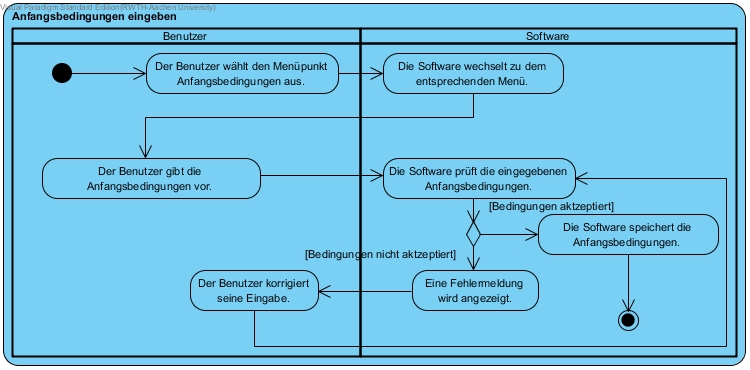
\includegraphics[scale=.5]{Bilder/Anfangsbedingungen_eingeben.jpg}\\
	\caption{Aktivitätsdiagramm Use Case Anfangsbedingungen eingeben}
	\label{Aktivitätsdiagramm Use Case Anfangsbedingungen eingeben}
\end{figure}

%Diskretisierungsgrößen eingeben
\begin{figure}[H]
	\centering
	%\hspace{-1.75cm}
	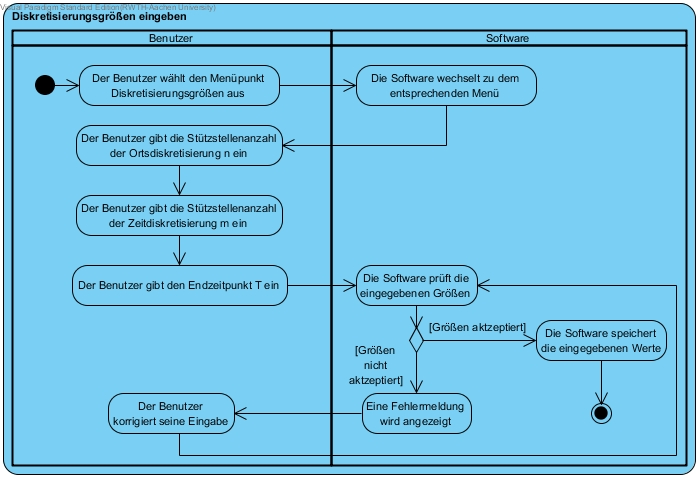
\includegraphics[scale=.5]{Bilder/Diskretisierungsgroessen_eingeben.jpg}\\
	\caption{Aktivitätsdiagramm Use Case Diskretisierungsgrößen eingeben}
	\label{Aktivitätsdiagramm Use Case Diskretisierungsgroessen eingeben}
\end{figure}

%Randbedingungen eingeben
\begin{figure}[H]
	\centering
	%\hspace{-1.75cm}
	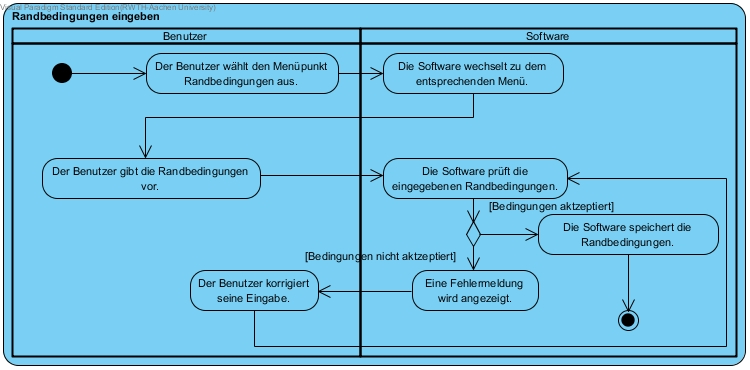
\includegraphics[scale=.5]{Bilder/Randbedingungen_eingeben.jpg}\\
	\caption{Aktivitätsdiagramm Use Case Randbedingungen eingeben}
	\label{Aktivitätsdiagramm Use Case Randbedingungen eingeben}
\end{figure}

%Simulieren
\begin{figure}[H]
	\centering
	%\hspace{-1.75cm}
	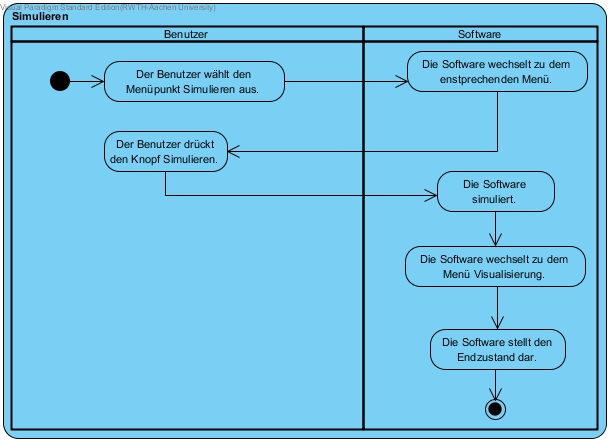
\includegraphics[scale=.5]{Bilder/Simulieren.jpg}\\
	\caption{Aktivitätsdiagramm Use Case Simulieren}
	\label{Aktivitätsdiagramm Use Case Simulieren}
\end{figure}

%Video abspielen
\begin{figure}[H]
	\centering
	%\hspace{-1.75cm}
	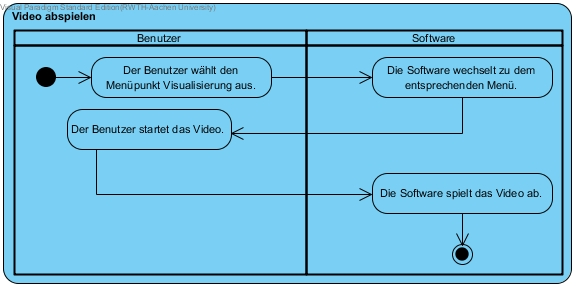
\includegraphics[scale=.5]{Bilder/Video_abspielen.jpg}\\
	\caption{Aktivitätsdiagramm Use Case Video abspielen}
	\label{Aktivitätsdiagramm Use Case Video abspielen}
\end{figure}

%Wärmeleitkoeffizienten eingeben
\begin{figure}[H]
	\centering
	%\hspace{-1.75cm}
	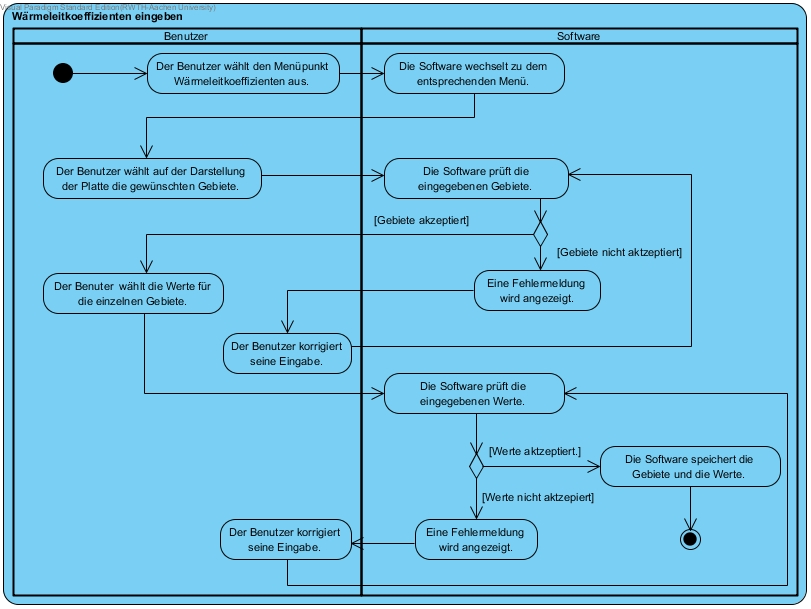
\includegraphics[scale=.5]{Bilder/Waermeleitkoeffizienten_eingeben.jpg}\\
	\caption{Aktivitätsdiagramm Use Case Wärmeleitkoeffizienten eingeben}
	\label{Aktivitätsdiagramm Use Case Wärmeleitkoeffizienten eingeben}
\end{figure}

%Wärmequellen eingeben
\begin{figure}[H]
	\centering
	%\hspace{-1.75cm}
	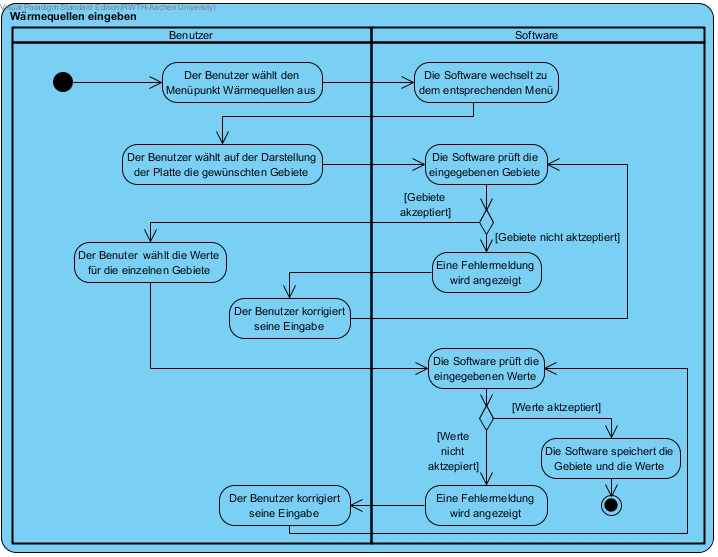
\includegraphics[scale=.5]{Bilder/Waermequellen_eingeben.jpg}\\
	\caption{Aktivitätsdiagramm Use Case Wärmequellen eingeben}
	\label{Aktivitätsdiagramm Use Case Wärmequellen eingeben}
\end{figure}

%Zustand anzeigen
\begin{figure}[H]
	\centering
	%\hspace{-1.75cm}
	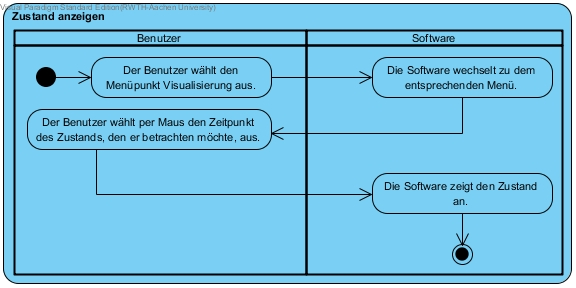
\includegraphics[scale=.5]{Bilder/Zustand_anzeigen.jpg}\\
	\caption{Aktivitätsdiagramm Use Case Zustand anzeigen}
	\label{Aktivitätsdiagramm Use Case Zustand anzeigen}
\end{figure}

\subsubsection{Systemanforderungen}
\subsubsection*{Funktionale Anforderungen}

\begin{enumerate}
	\item Der Benutzer kann mit linken Mausklicks Gebiete der Wärmeleitkoeffizienten eingeben und deren Werte per Tastatur festlegen.
	\item Der Benutzer kann mit linken Mausklicks Wärmequellen eingeben und deren Werte per Tastatur festlegen.
	\item Um das Problem zu spezifizieren,kann der Benutzer Funktionen für die Anfangs- und Randbedingungen vorgeben.
	\item Die Diskretisierungsparameter (Stützstellenzahlen der Orts- beziehungsweise Zeitdiskretisierungen sowie den Endzeitpunkt der Simulation) \& Simulationsparameter (Integrationsverfahren) können durch den Benutzer festgelegt werden.
	\item Die Simulation kann per Knopfdruck durch den Benutzer gestartet werden.
	\item Der Benutzer kann sich die zeitliche Entwicklung der Temperaturverteilung als Video oder einen Zustand als Standbild anzeigen lassen.
	\item Die Software kann durch den Benutzer per Knopfdruck auf den Ausgangszustand zurückgesetzt werden.
	\item Der Benutzer kann sich eine Hilfe zur Benutzung der Software anzeigen lassen.
\end{enumerate}

\subsubsection*{Nicht-funktionale Anforderungen}

\begin{enumerate}
	\item Dokumentation der Implementierung mittels Doxygen
	\item Grafische Oberfläche mit Qt
	\item Einfache Erweiterbarkeit um weitere Simulationsmethoden
	\item Lauffähig unter Windows und Linux (insbesondere auf dem RWTH Aachen Cluster)
	\item Grafische Oberfläche skaliert korrekt bei Veränderung der Fenstergröße
	\item Die Berechnung im Laufe der Simulation soll innerhalb von maximal 45 Sekunden abgeschlossen sein.
\end{enumerate}


\section{Begriffsanalyse}

\subsection{Klassenkandidaten}
\begin{itemize}
	\item Platte $\rightarrow$ Gitter
	\item Temperaturverteilung
	\item Temperaturkoeffizient ($\rightarrow$ durch \emph{Area} implementiert)
	\item Wärmequellen ($\rightarrow$ durch \emph{Area} implementiert)
	\item \textbf{Function}
	\item Startbedingung ($\rightarrow$ durch \emph{Function} implementiert)
	\item Randbedingung ($\rightarrow$ durch \emph{Function} implementiert)
	\item Endzeitpunkt, Stützstellenzahl (Ort- \& Zeitdiskretisierung)
	\item Simulation
	\item Problem + Ergebnis $\rightarrow$ \textbf{Model}
	\item Zustand/Video
	\item Fehlermeldung ($\rightarrow$ durch GUI implementiert)
	\item \textbf{Area}
	\item \textbf{IntMethod} $\rightarrow$ \textbf{ImpEuler}, ...
	\item \textbf{IterativeSolver} $\rightarrow$ \textbf{Jacobi}, ...
\end{itemize}

\subsection{Begriffsnetz}
Abbildung \ref{Begriffsnetz} zeigt das Begriffsnetz.
\begin{figure}[H]
	\centering
	%\hspace{-1.75cm}
	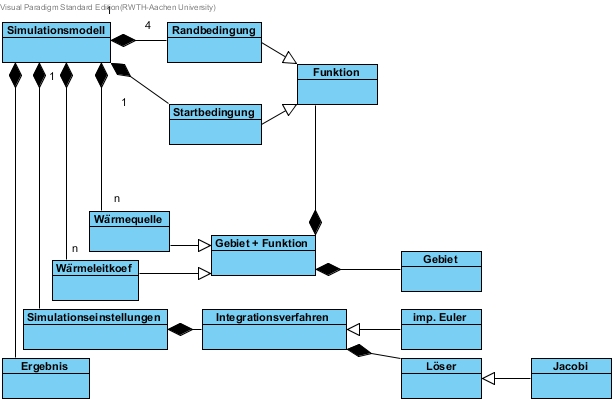
\includegraphics[scale=.75]{Bilder/Begriffsnetz.jpg}\\
	\caption{Begriffsnetz}
	\label{Begriffsnetz}
\end{figure}